\chapter{Thrust 0: \Cyclus Infrastructure Development}\label{chap:thrust0}

Under Thrust 0, the \Cyclus framework was advanced from a conceptual design to
a fully functional software tool.  As this project began, the fundamental
features of \Cyclus were in place, but it was far from a usable tool for fuel
cycle simulation.  Through the efforts of this project, \Cyclus emerged as a
more usable and stable software platform for nuclear fuel cycle analysis.  The
overarching goal was to provide maximum flexibility so that changes in fuel
cycle design did not require substantial retooling of the software.  Specific
design features that support this flexibility include:
\begin{enumerate}
\item \textbf{Modular design} to support extensibility with runtime swappable facility models.
\item \textbf{Agent-based approach} to incorporate social/behavior interaction models to govern how each facility interacts with others.
\item \textbf{Individual facility modeling} to allow each facility to operate in a distinct manner, allowing modeling of startup, shutdown and other disruptions.
\item \textbf{Discrete material tracking at the nuclide level} to capture the effects of individual facility performance and enable forensic tracking of material object ownership.
\item \textbf{Minimal physics assumptions} to enable different users to invoke low fidelity, systems level models or high fidelity, facility level models, or anything in between.
\end{enumerate}

Under this project, the \Cyclus effort developed into an \textit{ecosystem} composed of:
\begin{itemize}
\item an open source simulation kernel, known as \Cyclus,
\item many plug-in modules, each implementing a particular model for a
  facility, institution or region, and known as \textit{archetypes}, and
\item an open source analysis and visualization tool, known as Cyclist.
\end{itemize}

The first section of this chapter will describe the fundamental design and
implementation of the \Cyclus kernel while the following section will describe
the infrastructure to support the development of new archetypes.

\section{Fundamental Design and Implementation} %%fundamentals paper

More details regarding the implementation and demonstration of the fundamental
design of the \Cyclus kernel are available in ref
\citeprod{huff-fundamentals}.

\subsection{Modularity}

The modular nature of \Cyclus is a key element to its ability to remain
flexible, and also drives many subsequent design decisions.  The main goal of
this flexibility is to allow for the computational models that represent
individual agents (see Section \ref{sec:abm}) to be swapped easily, as a
user option.  Two specific advantages of this choice are that (a) individual
researchers can focus their efforts on new modules that match their expertise
and support their needs, and (b) the impact of changing modeling choices can
be explored in a consistent environment by swapping only one module at a time.

In its purest expression, each module operates in a so-called
\textit{black-box} fashion.  That is, any single module has no knowledge of
the internal state or behavior of any other module and can only interact in a
narrowly defined and specific way.  In addition to imposing a number of
software engineering limitations on the implementation of the kernel and
archetypes, this design goal also requires careful design of that interaction
interface among the modules.

Figure \ref{fig:framework} illustrates this concept, indicating the different
\gls{API} for each type of agent, and the possibility of different
implementations in each case.  Different implementations of each type of
facility, for example, may use different models to describe the physics and/or
the interaction behavior of that facility.  These differences can represent
small perturbations from other implementations or entirely different
approaches, including wrapping other software.  Because the modules can be
swapped at runtime, without requiring the software to be recompiled, this also
facilitates different distribution modes for these modules, as shown in Figure
\ref{fig:modifiedopen}, including fully open source, export controlled, and/or
proprietary commercially licensed modules.

\begin{figure}[htbp]
  \centering
  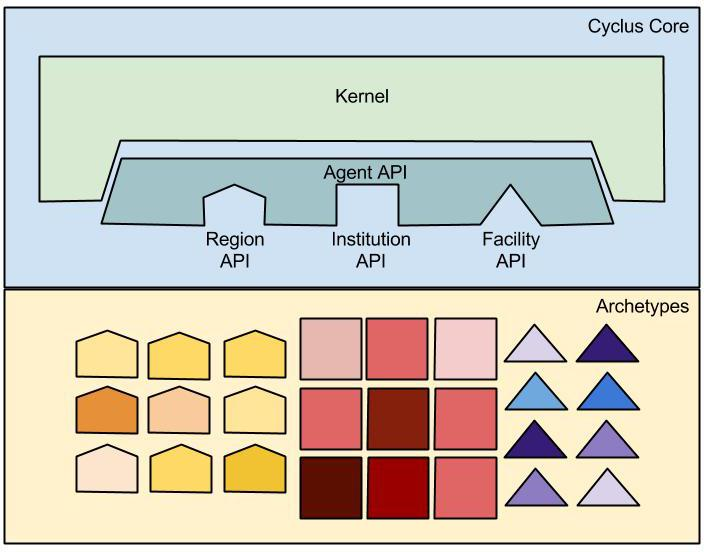
\includegraphics[width=0.7\columnwidth]{./images/framework}
  \caption[The \Cyclus core provides \glspl{API} that abstract away the details in
    the kernel and allow the archetypes to be loaded into the simulation in a modular
    fashion.]{The \Cyclus core provides \glspl{API} that abstract away the details in
    the kernel and allow the archetypes to be loaded into the simulation in a modular
    fashion. \citeprod{huff-fundamentals}}
  \label{fig:framework}
\end{figure}

\begin{figure}[htbp]
  \centering
  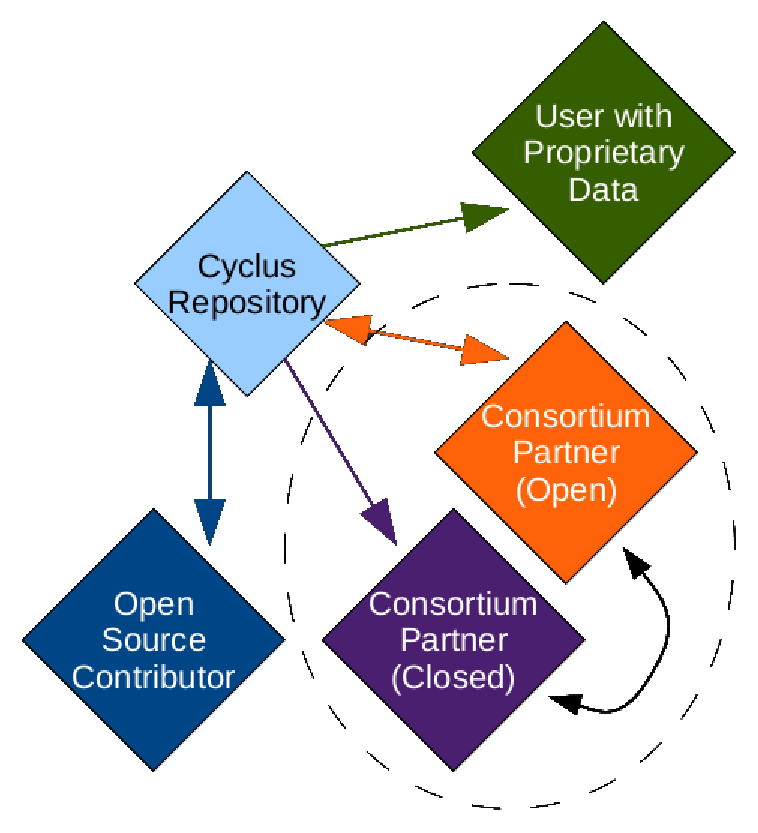
\includegraphics[width=0.5\columnwidth]{./images/modifiedopen.eps}
  \caption[The \Cyclus framework enables fully open, partially open, and fully
    closed collaborations.]{The \Cyclus framework enables fully open, partially open, and fully
    closed collaborations\citeprod{Carlsen2016}.}
  \label{fig:modifiedopen}
\end{figure}


\subsection{Agent-based Paradigm}
\label{sec:abm}
% superior detail in capturing simulation dynamics
% more flexible control over behavior
% describe Region/Institution/Facility hierarchy
% note importance of generic resource exchange paradigm

\Cyclus implements an \gls{ABM} paradigm.  In addition to being a natural
consequence of the modularity described above, the \gls{ABM} paradigm is more
flexible and intuitive (from both a developer and user perspective) than the
system dynamic approach used in current simulators.  System dynamics is a
popular approach for modeling nuclear fuel cycles
\citeref{jacobson_vision_2009,van_den_durpel_daness_2009,guerin_impact_2009,guerin_benchmark_2009}.
Formally however, system dynamics models are simply a strict subset of
agent-based models \citeref{macal_agent-based_2010}.  That is, any system
dynamics model can be translated into an agent-based model.  \gls{ABM}
techniques therefore enable a broader range of simulations in a more generic
fashion.

To ensure interchageability, all agents are based on a common set of
object-oriented \glspl{API} defined as part of the \Cyclus kernel that define
how they interact with other agents and with the environment.  These
\glspl{API} standardize and simplify the implementation of required agent
behavior such as trading resources.  Optional \textit{mixins} are also
provided in a toolkit to provide community standards for some optional
behaviors.  More details on archetype development are in Section
\ref{sec:archetypes}.

\Cyclus provides a novel representation of entities in the nuclear fuel cycle
that reflects the reality in international nuclear power: \textit{facilities}
implementing individual fuel cycle technologies, \textit{institutions}
managing those facilities, and \textit{regions} providing geographical and
political context for institutions and facilities.  Under this paradigm,
regions and institutions are first class agents much like facilities: they can
be developed as stand-alone modules to implement different behaviors and
swapped at runtime.  \Cyclus implements a \gls{RIF} relationship through a
parent-child hierarchy where regions are the parents of institutions which
are, in turn, the parents of facilities.  In this structure, institutions are
typically responsible for making decisions to deploy and decommissioning
facilities, while regions are typically responsible for establishing an energy
demand.  Both regions and institutions can have an impact on inter-facility
resource flow during the resource exchange process.

\subsection{Discrete Objects}
% enables more realistic models and metrics
% material routing metrics
% shadow fuel cycles
% etc.

Implied by this \gls{ABM} paradigm is that \Cyclus models facilities,
institutions, regions, and resources as discrete objects, allowing for a range
of modeling granularity.  This is in contrast to the fleet-based approach used
in most other fuel cycle simulators, although it is possible to implement
\Cyclus archetypes that represent fleets of identically behaving
facilities\citeprod{carlsen_fleet}.  This discrete facility capability is
necessary to enable the tracking of discrete material objects.  Examples of
use cases supported by discrete material tracking include spent fuel storage,
transport and disposal models that require representation of discrete casks
and the individual isotopic compositions of their contents.

Another such use case seeks to capture system vulnerability to material
diversion. Provenance and trade-history of distinct materials is the
fundamental information unit in such studies, and so this type of analysis
requires discrete simulation of a target facility and the individual materials
modified within it.  Material risk analysis, therefore, demands that both
facilities and materials should be discretely modeled objects like those in
\Cyclus.

\Cyclus represents these discrete tradable objects generically as
\textit{resources}, with a specific implementation for \textit{materials} to
represent typical nuclear materials with a mass and nuclide composition.
Typical operations on material objects, e.g. splitting, combining, decay,
\emph{etc.}, are tracked in detail to support simulation wide mass
conservation.  The history of ownership and transfer of each object is also
tracked.

Material objects in \Cyclus can have compositions with an arbitrary number of
nuclides and can be optionally subject to radioactive decay, either at the
discretion of the facilities which own/manage the material, or whenever it is
observed/traded in the simulation.  In large simulations, this tracking of
discrete material objects can lead to many objects that change frequently.  A
number of implementation details exist to minimize the impact on system memory
and output database file size.

A critical capability at the intersection of the swappable archetype and the
discrete resource object paradigms is the \gls{DRE} which implements a market
mechanism at each time step for matching consumer agents' requests for
material with supplier agents' offers for material.  The \gls{DRE} is
described in detail in Ref \citeref{gidden_agent-based_2015}.  Supporting the
general \Cyclus philosophy, facilities are treated as black boxes and a
supply-demand communication framework is defined.  The primary development of
the \gls{DRE} was supported under a different project and is reported
there\citeref{cyclus-opt-report}.

The \gls{DRE} is a novel simulation concept in the nuclear fuel cycle domain. It
provides a flexible supply-demand infrastructure, supporting dynamic flows of
resources between agents, even as those agents enter and leave the simulation, and
even when those agents are defined by archetypes of arbitrary complexity. Trading
between agents can be affected by both the
proposed quality of a resource and agent relationships through the use of
preferences. Accordingly, a wide range of possible effects can be
modeled, from capacity-limited fuel supply to international trade agreements.

\subsection{Simulation Support}
So that users and developers can build working simulations in the shortest time
possible, the \Cyclus ecosystem provides fundamental building blocks: basic
archetypes and a toolkit of commonly needed functions.  The \Cycamore library
provides a suite of fundamental Region, Institution, and Facility archetypes,
while the \Cyclus toolkit provides assistance to developers.

\Cycamore \citeprod{carlsen_cycamore_2014}, the \Cyclus additional module
repository, provides a fundamental set of dynamically loadable libraries
providing agent archetypes for basic simulation
functionality within \Cyclus.  Since \Cyclus relies on external
archetypes to represent the agents within a simulation, \Cycamore provides the
basic archetypes a new user needs to get started running simple simulations.
These archetypes support a minimal set of fuel cycle simulation goals and
provide, by example, a guide to new developers who would seek to contribute
their own archetypes outside of \Cycamore.

As of version 1.5, \Cycamore contains one region archetype, two institution
archetypes, and eight facility archetypes. Short descriptions of these functions can be found in
Table \ref{tab:cycamore}.

\begin{table*}[ht]
\centering
\caption[The Archetypes in \Cycamore seek to cover a large range of simple
simulation use cases.]{The Archetypes in \Cycamore seek to cover a large range of simple
simulation use cases\citeprod{carlsen_cycamore_2014}.}
\label{tab:cycamore}
\begin{tabularx}{\textwidth}{rlX}
\hline
\textbf{Type} & \textbf{Archetype Name} & \textbf{Functionality} \\
\hline
Facility & EnrichmentFacility & This facility enriches uranium at a specified capacity. \\
Facility & FuelFab & This facility fabricates fuel material based on separated streams. \\
Facility & Reactor & A reactor model that handles batch refueling, based on pre-determined recipes of compositions. It requests any number of input fuel types and transmutes them to static compositions upon discharge.\\
Facility & Separations & This facility separates an incoming material into specified streams. \\
Facility & Storage & This facility holds incoming material for a specified time until before it is offered. \\
Facility & Mixer & This facility combined a set of incoming streams into a single stream. \\
Facility & Sink & This facility is capable of accepting a finite or infinite quantity of some commodity produced in the simulation. \\
Facility & Source & This facility generates material of the composition and commodity type specified as input.  \\
Institution & ManagerInst & The manager institution manages production of commodities among its facilities by building new ones as needed. \\
Institution & DeployInst &  This institution deploys specific facilities as defined explicitly in the input file. \\
Region & GrowthRegion & This region determines whether there is a need to meet a certain capacity (as defined via input) at each time step. \\
\hline
\end{tabularx}
\end{table*}

In addition to the core functionality of the \Cyclus kernel, which is focused
on the set of capabilities needed to implement an agent-based simulation with
\gls{DRE}, a toolkit is provided to assist developers and users with robust
and standardized implementations of related simulation and nuclear engineering
tasks. The toolkit is an actively developed part of \Cyclus, with a primarily
forward-looking focus on supporting interesting \textit{in situ} metric
analysis tools.  The toolkit contains methods to support demand-constrained
facility agent deployment with methods that describe different shaped curves
for electricity demand, and then assess the available capacity relative to
those demand curves, deploying new facilities when necessary.  The toolkit
also includes nuclear engineering specific methods, such as models to
calculate the relationship between material quantity, quality and enrichment
capacity.

\subsection{Quality Assurance}

To garner the trust of a broad user and archetype developer community, the
\Cyclus project must implement a strategy to assure the ongoing quality of the
software it provides.  Multiple strategies, collectively known as
\emph{\gls{QA}}, have been developed by the scientific software development
community to mitigate structural and algorithmic errors in software.  \Cyclus
has adopted the best practices of the open source software community for
ensuring software quality including:
\begin{itemize}
\item version control: careful control and cataloging of changes to the
  software with full attribution of each change to each author,
\item code review: every individual change is reviewed by another developer
  for many aspects, from style to algorithmic performance to correctness, and
\item continuous integration: automated testing of individual software units
  and integrated solutions as each change is proposed and incorporated.
\end{itemize}
Ref \citeprod{huff-fundamentals} provides more details on each of these topics.


\section{Facilitating Archetype Developers} %% Archetype paper
\label{sec:archetypes}

A principal distinguishing feature of \Cyclus is the ability to introduce
novel agents by developing customized archetypes.  Not only is this a
departure from the structure of most \gls{nfcs} tools, but
the degree of specialization that is necessary to represent different fuel
cycle facilities is a departure from many agent-based simulation frameworks.
Each agent must interact with the \Cyclus kernel and other agents using a rich
interface that controls initialization of agent parameters, agent interaction
with the \gls{DRE}, initiation of agent behavior between trades,
decommissioning of agents, and recording of all agent data.  Correct
implementation of these interactions with the kernel are necessary, in
addition to implementing the physics and interaction behaviors that are the
true motivation for the new agent archetype.

To mitigate the difficulties of writing archetypes, \Cyclus aids in overcoming
the hurdle of interfacing with the kernel itself. Additionally, to the extent
possible, \Cyclus should also provide tools that ease the implementation of
the physics and desired behavior.  A variety of strategies are used by \Cyclus
to ease archetype development:

\begin{itemize}
\item \textbf{Automatic Model Templating:} By automatically inspecting and
  creating portions of archetypes, the overhead of adhering to the \Cyclus
  \gls{API} is removed. This is performed via preprocessing archetypes and
  then automatically generating the necessary C++ source code to implement
  many parts of the necessary interface.

\item \textbf{Data Communication Protocol:} \Cyclus provides a common basis
  for archetypes to store and retrieve complex data in its database. This is
  achieved through the implementation of \Cyclus-specific type system.  This
  alleviates the need for archetype developers to invent and implement custom
  solutions for storing the data that is generated by the archetype.

\item \textbf{Metadata Annotations:} Archetypes have a standard place to store
  and retrieve both pre-defined and arbitrary metadata.  This allows for
  archetype developers to communicate relevant information to tools outside of
  \Cyclus (such as a visualization tool).

\item \textbf{Input Validation:} \Cyclus uses an \gls{XML} input file format
  because it allows for a the definition of a schema that can be used to
  automatically validate the input file.  The schema for each archetype is
  automatically generated by the \Cyclus tools, relieving the developer of
  this burden while still allowing them to impose automatic validation.

\item \textbf{Model Location:} \Cyclus has a packaging system for archetypes
  and libraries of archetypes. This provides a standard mechanism for
  searching for and locating models on a user's system.  Furthermore, all
  archetype developers can uniquely specify their own archetypes without the
  fear of overlapping names.  For example, two developers could each have a
  \texttt{Reactor} archetype, but they would exist in different packages and
  be disambiguated.

\end{itemize}

Though the above mechanisms are discussed with respect to \Cyclus, they are
transferable to any agent-based modeling framework that requires modular agent
archetypes. The following subsections present greater detail regarding these
strategies.  Further detail and examples are available in
Ref. \citeprod{DBLP:journals/corr/ScopatzGCFHMORW15}.

\subsection{Automatic Model Templating}
\label{sec:code_gen}

Every \Cyclus archetype is required to implement a standard set of member
functions that control the definition of a prototype that is derived from that
archetype (\texttt{InfileToDb}), the life cycle of each instance of that
archetype (\texttt{InitFrom},\texttt{Clone},\texttt{InitInv}), and the
interaction of the agent with the database that stores the state of each agent
(\texttt{Snapshot},\texttt{SnapshotInv}).  There are additional option
functions that allow an archetype to take specific action when it is deployed
(\texttt{Build}, \texttt{EnterNotify}), when it chooses to deploy or
decommission its own children (\texttt{BuildNotify},\texttt{DecomNotify}), or
when it is decommissioned itself (\texttt{Decommission}).

Since each archetype is free to define a unique and independent set of member
data and behaviors, these methods must be specific to the archetype so that
they can be sure to address all the correct data members.  Manually generating
all of these functions is tedious, time consuming, error prone, and may
require specialized knowledge of the \Cyclus kernel that would be otherwise
unnecessary.  It is, however, possible to automatically generate the code that
implements the above functions based on the set of members that are defined in
the archetype.  Furthermore, with a small amount of additional metadata (see
Section \ref{sec:metadata} below) for each member variable, it is also
possible to automatically generate the correct \gls{XML} schema for validation
of input to that archetype.

A custom pre-processor, called \texttt{cycpp}, has been written to read and
parse the simplified definition of an archetype and automatically generate the
correct methods to implement the above interface.  The pre-processor replies on
metadata that is attributed to the member data through the use of
\texttt{\#pragma cyclus} directives.  These are otherwise skipped by the
compiler, but can be used to identify special behavior.

\subsection{Data Communication Protocol}

\Cyclus relies on a number of alternative storage formats for the data it
generates, allowing the user to prefer either typical \gls{SQL} databases or
numerically oriented \gls{HDF5} files.  Both of these systems have full
support for simple data types, but much of the data generated in a fuel cycle
simulation has more complex relationships.  The \Cyclus kernel has implemented
an extensible system to support complex types.  This is important for
archetype designers/developers because it allows them to use a richer and more
expressive set of data structures, and reduces possible errors that might be
introduced by having to transcribe those data structures in/out of simpler
forms for storage.  This is also an important feature to enable automatic
model templating: \texttt{cycpp} is able to determine the ``shape'' of complex
data structures and invoke the correct tools for storage of that data.

\subsection{Metadata Annotations}\label{sec:metadata}

As mentioned above, automatic code generation relies on metadata that is
either determined automatically from the archetype declaration or is
introduced in optional \texttt{\#pragma cyclus} directives.

One use of this metadata is to define the behavior of archetype member data,
and provide a high-level mechanism to invoke many low-level behaviors through
the \texttt{cycpp} pre-processor.  For example, a simple declaration of the
shape of a data type can be used to generate the code that will invoke the
correct data storage behavior in various formats.

All metadata, whether required or optional, is stored as part of the archetype
and available during a \Cyclus simulation for general use.  At a fundamental
level, this allows for reflection in a way that is not typical of C++
software: the archetypes are aware of their own name and the types of their
member variables.

Finally, the annotations can be particularly valuable beyond the \Cyclus
kernel.  \Cyclus provides a mechanism to query those annotations for use in
other tools that support input file generation and output visualization.
Several standard annotations are available to support input file generation,
including declaring a default value, different forms of documentation, and
physical units.  Use of this data will be discussed further in Chapter
\ref{chap:thrust3}.

\subsection{Input Validation}

A \Cyclus input file consists largely of the definition of agent
\textit{prototype}, each formed by configuring an archetype with a set of
parameters.  In many software tools that rely on user input, validating that
the users choices for those parameters makes sense in some way can be a
substantial task.  This kind of validation includes checking whether certain
values are within physical bounds, whether all values are defined with the
correct type, and whether there are enough entries for complex data types.  By
relying on \gls{XML} as the input file format, \Cyclus is able to invoke its
built-in grammar-based validation capability.  A \emph{schema} provides a
definition of the correct grammar against which the input file is tested.

In most cases, the schema for an archetype can be automatically generated from
the archetype declaration, with some additional information collected from
annotations.  This allows archetype developers to have the full advantage of a
grammar-based validation without having to learn the details of how those
grammars are defined.  Grammar for the validation of data type and structure
can be derived by inspecting the type and structure of the member variables
themselves.  Grammar that validates against specific semantic meanings (e.g. a
variable must be positive) requires metadata annotations.  The metadata
annotations also provide a mechanism for developers to completely override the
auto-generation of the schema.

\subsection{Model Location}\label{sec:model_location}

The final capability provided to archetype developers is a standardized way to
declare the location of a specific archetype.  Since archetypes are
dynamically loadable, it is necessary for the \Cyclus kernel to find each
archetype at runtime.  The simplest strategies for finding archetypes rely on
them all being named in a standard way in a standard location in the
file system.  This is both constraining and presumes a level of coordination
among archetype developers that undermines the flexibility of the plugin
archetypes.  Instead, an archetype specification mechanism has been developed
to allow both flexibility and disambiguation of archetypes at runtime.  The
specification allows a user to define where in the file system a plugin library
is located, the name of that library, and the name of the archetype within
that library.  This means that different developers can choose the same name
for their library of archetypes, as long as it is stored in a different
location.  Similarly, they can have similar names for their individual
archetypes without worrying about name collision.


This set of tools and capabilities not only lowers the barrier to the
development of new archetypes, allowing developers to focus on the specific
physical and behavior models of interest to them.  The software development
tasks of agent instantiation, data persistence, and input validation are
handled automatically.  This allows the \Cyclus ecosystem to use advanced
technologies for these purposes without raising the cognitive burden on
archetype developers to learn all of those technologies.

\section{Summary}

This project enabled the \Cyclus effort to develop into a robust tool for fuel
cycle simulation, meeting its primary design goals while also facilitating
contributions from a wide set of archetype developers.  This product of Thrust
0 was a next-generation fuel cycle simulation framework suitable for the user
experience extensions studied in the other thrusts of this project.
